\chapter{Simulation-Driven Optimization of Slot Antenna using Genetic Algorithm}
\label{chap:chap3}
\section{Introduction}\label{c3sec_intro}
Microstrip antennas were the first printed patch antennas. The concept of microstrip antennas was first proposed in 1953 by G. A. Deschamps et al. \cite{mpa00}. Microstrip antennas and arrays were practically fabricated in the 1970s in several contemporary works such as \cite{mpa02} and \cite{txmPhasedArray}. The design trends until the beginning of the 1980s were covered in a survey work by K. R. Karver et al \cite{mpaSurvTech}. This review gives significant insights into the design trends until that period. The number of works related to microstrip antennas increased exponentially over the years after 1980 \cite{mpaHist01}. The designing of microstrip antenna arrays was another trend that evolved almost simultaneously. At that time, microstrip antennas were known for their disadvantages of low gain and bandwidth. This may be a reason why many researchers considered the design of compact, rigid and planar arrays using microstrip antennas to enhance the gain. In 1974, a phased array of microstrip antenna elements was proposed by R. F. Munson \cite{txmPhasedArray}.

In the initial phase, most of the works on microstrip antennas were related to feeding mechanisms. These works were based on some simplifying approximations for making them computationally simple. These models provide useful information regarding impedance, radiation patterns, efficiency and bandwidth of the antennas \cite{mpaReview1992}. The two most commonly used feeding mechanisms for microstrip antennas are the microstrip line feed and the coaxial feed. These two techniques are widely in practice since the 1970s.

Between the mid-1970s and early 1980s, for the first time, several research works reported the design and modeling of microstrip antennas. The transmission line model and the cavity model were formulated during this period \cite{handbook}. The generalized transmission line model and the generalized cavity model were proposed in the the 1980s, which extended the transmission line model and the cavity model respectively to include microstrip antennas with more complex shapes \cite{handbook}. Finally, with the availability of modern computers, full-wave electromagnetic solvers were created. By the 1990s there were commercially available full-wave electromagnetic solvers. This led to a remarkable increase in the volume of research publications in the field of antenna design. Antennas with highly complex geometrical structures can be easily designed and simulated using software applications such as HFSS{\circledR}, CST{\circledR}, etc \cite{practGuide3D}. Antennas of various sizes and shapes were designed during this period \cite{smallPatch0, BandSize0, HPatch1, uslot1, dualBandCircPol, dualBandWLAN, fractal1, slottedUWB, bandnotchCSRR1, bandnotchEBG1, SlottedPatchModel, spiralSlotGnd, GndSRRPatch}. The analytical modeling and parameterizations of antennas, on the other hand, became less popular. The few analytical works published in this period were primarily concerned about developing an overall understanding of the antenna rather than formulating a design methodology. The designs are mostly validated from simulation and measurement results.

Equivalent circuit modeling of antennas is a more recent approach to antenna modeling. In this approach, the antenna is modeled as an RLC network \cite{rectEqCkt, Broadband_EqCkt, UwbEqCktMethod, UwbPmaEqCkt1, UwbPmaEqCkt2, UwbPmaEqCkt3, UwbPmaEqCkt4, UwbNotchEqCkt}. The representation of the input impedance is a challenging task in equivalent circuit modeling. Results obtained from a high-fidelity full-wave model are often used for setting and tuning the parameters of an equivalent circuit model.

In recent years, soft-computational optimization algorithms are becoming popular for the design of microstrip antennas and arrays \cite{UwbPmaGaFdtd, cadNASA, compCAD4Arry, antSurrD01, surrMTM01, antSurrConstMO}. Soft-computational designs involve iterative adjustment of the geometrical parameters of an antenna using a soft-computational optimization algorithm to obtain optimized values of the performance parameters such as resonant frequency, gain, bandwidth, etc. The process requires the computation of the electromagnetic parameters of an antenna at each iteration of the optimization algorithm. The full-wave methods are computationally very expensive and time consuming for iterative computation. Surrogate models have emerged as a solution to this problem.

In \cite{patch_miniaturize_ga}, the dimensions of a rectangular patch antenna are optimized using genetic algorithm (GA). Five physical dimensions of the antenna are tuned algorithmically to optimize the antenna. This is a 5-dimensional continuous problem. Here, the antenna is simulated in CST studio in order to calculate the cost function and the genetic algorithm is implemented in MATLAB.

In \cite{freqReconfCogn} a similar approach is presented using GA for designing an antenna for cognitive ratio application. In this work, the shapes of the slots and the locations of the switches in the ground plane are optimized for adjustment of the bandwidth. Here, the switches in the ground plane help in exciting the antenna at different modes. Each mode has its own resonance frequency. The antenna can be tuned to resonate at different frequencies with the help of the switches. The optimization problem was aimed to minimize the number of switches so that the same dynamic range of the resonant frequency of the antenna can be obtained with a minimum number of tunable parameters.

One of the earliest works that reported the use of evolutionary-based approaches in the design of a metamaterial unit cell is \cite{optMtm}. Here, genetic algorithm is used to design a metametarial unit cell with negative value of $\mu$. This is a discrete problem where the final structure is constructed by iteratively filling the area with small structural elements. A similar work for design of metamaterial unit cell using topology optimization is reported in \cite{lh_mtm}.

Soft-computational algorithms are also widely used for the design of arrays. Array optimization includes a wide range of applications such as array synthesis \cite{arraySynth1, arrayThin1}, array optimization \cite{arraySynth3}, side lobe level (SLL) reduction \cite{arraySynth2, arraySynth4}, etc. In \cite{compCAD4Arry}, a comparison of genetic algorithm (GA), particle swarm optimization (PSO), and differential evolution (DE) is presented in terms of their application in the optimization of planar arrays.

Traditionally, computational tools such as Matlab or Python are used for implementing optimization algorithms, whereas antennas are simulated with commercially available full-wave solvers such as AEDT (or HFSS), CST studio, etc. Setting up different software applications together in order to perform the optimization is a computationally intensive task. AEDT provides an Iron-Python script interface which can be used for automating certain simulation tasks. It is a limited implementation of Python that lacks support for many packages, crucial for implementing computationally intensive algorithms. Here, the genetic algorithm is implemented with Iron-Python that functions within AEDT and does not need any external libraries to be installed.

The remaining part of this chapter are arranged as follows. Section \ref{c3sec-prop-alg} contains the details of the proposed method for implementing the genetic algorithm in AEDT. Section \ref{c3sec-exp-details} covers the details of the experiment formulated to test the proposed approach. The experimental results are discussed in Section \ref{c3sec_expt-res}. Finally, the chapter is concluded in Section \ref{c3sec_concl}.

\section{Details of the Proposed Algorithm} \label{c3sec-prop-alg}
\begin{figure}
  \centering
  \includegraphics[width=0.6\linewidth]{bc-flowchart.eps}\\
  \caption{Flowchart of the implementation of genetic algorithm in AEDT}\label{fig1}
\end{figure}
Genetic algorithm is a bio-inspired optimization algorithm. It is a global-search algorithm that mimics the principle of natural selection to arrive at a global maximum point in the search space. The algorithm iteratively generates samples to minimize the error, given by a cost function. This section provides the details of how the cost function is formulated in an antenna optimization problem followed by the details of the genetic algorithm and its various terms in the context of antenna optimization.

\subsection{Cost Function for Antenna Optimization}
In case of antenna optimization, the cost function is derived from the performance parameters of the antenna such as resonant frequency, bandwidth, far-field gain etc. The variables to be optimized are the physical dimensions of the antenna such as length, width, position of the feed etc. The cost function yields the difference between the actual and the desired performance of the antenna. For example, if the design goal is to obtain resonance at a particular frequency, the cost function will be:
\begin{equation}
E = \left|f_{\textrm{target}}-f_{\textrm{obtained}}\right|
\end{equation}

If the desired antenna has two resonant frequencies $f_1$ and $f_2$, the goal is to minimize the return loss ($S_{11}$) parameter at these two frequencies. Accordingly, the cost function may be formulated as follows.
\begin{equation}
E = \max\left(S_{11}(f_1), S_{11}(f_2)\right)
\end{equation}
If the goal is to maximize the far-field gain, the cost function will be
\begin{equation}
E = \left|G_{\textrm{target}}-G_{\textrm{obtained}}\right|
\end{equation}

In order to calculate the error using the cost function, it is important to evaluate the performance of the antenna corresponding to the generated set of dimensions of the antenna. Full-wave electromagnetic solvers are the most reliable tools for this purpose. Fig. \ref{fig1} shows the flowchart of the technique used for implementing the genetic algorithm for optimizing antennas with AEDT. The dimensions are initialized arbitrarily. The genetic algorithm then iteratively updates the dimensions to minimize the error given by the cost function. The cost function depends on the design goals.

\subsection{Genetic Algorithm for Antenna Design}
The term ``Genetic algorithms'' refer to a number of implementations of an optimization algorithm inspired by the law of natural selection. Many of these techniques are discussed in \cite{gaBook}. In the present work, the implementation of genetic algorithm is inspired by the algorithm reported in \cite{gaImpl}. This section breaks down the genetic algorithm terminologies in a way to fit into the context of antenna optimization.

Like any other soft-computing technique, genetic algorithm also has some hyper-parameters that must be pre-defined for the given problem. The hyper-parameters of a genetic algorithm includes the DNA size, population size and the number of generations. The dimensionality of the optimization problem is represented by the DNA size. It is equal to the number of dimensions that are to be optimized. The maximum number of iterations to be performed before terminating the optimization process is represented by the number of generations.

Most of the terminologies used in genetic algorithm are directly borrowed from biology. These are generalized terms and it is important to understand their meanings to be able to relate these terms with the optimization problem that need to be solved. Some terminologies of genetic algorithm and their interpretation in terms of antenna optimization are discussed as follows.

\begin{itemize}
\item \textbf{Selection of the initial population:} The initial population is an array of random values of the dimensions of the antenna. Each element of the array is another array of the size equal to the DNA size. For example, if four physical dimensions of the antenna are to be optimized using genetic algorithm, the initial population will be $N$ arrays each having four elements. Each array is called a chromosome. A chromosome, thus is a possible solution to the optimization problem. Each element of a chromosome is called a DNA and it corresponds to a particular physical dimension of the antenna that needs to be optimized.
\item \textbf{Assigning Weights to the Chromosome:} The fitness of a chromosome is inversely related to its cost function. If the cost function of a particular set of dimensions is high, it has a low fitness. Thus, for every chromosome, the full-wave simulation is to be executed in order to obtain its electromagnetic parameters. This is the reason why the genetic algorithm has a very high time consuming when used to solve an antenna optimization problem. If the cost function of a particular solution is $c$, its fitness value is considered as $1/c$. This fitness value is assigned as its weight.
\item \textbf{Weighted Selection:} This is the step where chromosomes are selected for the next generation (iteration). Two sets of dimensions are selected that has the maximum fitness value. If the fitness is greater than a threshold, the optimization process is terminated and the available solution with the maximum fitness is the optimal solution to the problem. If the fitness of all the chromosomes is less than the threshold, a chromosome with the maximum fitness is used to obtain the next generation. In case of antenna optimization, a set of dimensions is selected in this step that has the minimum cost function in terms of the given design criteria.
\item \textbf{Mutation:} Mutation is the process by which the next generation is obtained from the chromosome selected in the previous step. A small random number is added to each physical dimension (DNA) of the chromosome in order to obtain the next generation. In other words, each physical dimension of the antenna leading to the minimum value of the cost function is slightly distorted to obtain the next generation.
\item \textbf{Crossover:} In some optimization problems, the next generation is obtained by combining a pair of two chromosomes with minimum loss. In this case, some DNAs from one chromosome and some DNAs from the other chromosomes are interchanged at different positions. This technique, however, is not always suitable for antenna optimization. Each dimension of the antenna has a particular range. Hence, two DNAs corresponding to two different physical dimensions cannot be interchanged to perform a crossover. That is why crossover is not performed in the present work.
\end{itemize}

\begin{figure}[h]
\centering
\includegraphics[width=0.9\linewidth]{bc-ga-flow.eps}
\caption{Flow diagram of the implementation of genetic algorithm for antenna optimization.}\label{ga-flow}
\end{figure}

The steps discussed are presented as a flowchart in the context of antenna design in Fig. \ref{ga-flow}. Here, all terminologies of genetic algorithm are replaced by antenna design terminologies in order to make the process easily relatable to the context of antenna design. Crossover is not performed in this case and the next generation is obtained from the set of dimensions with the minimum value of the loss function through the process of mutation by adding some small random numbers.

\section{Experimental Details} \label{c3sec-exp-details}
This section covers the details of an experimental evaluation of genetic algorithm for optimizing a printed antenna. The method discussed in the Section \ref{c3sec-prop-alg} is used here to optimize an H-shaped slot antenna. Slot antennas are printed antennas. Unlike microstrip antennas, the slot antenna has a slotted section etched from the ground plane. Slot antennas are excited with a microstrip line present at the opposite face of the PCB. Coplanar wave-guide (CPW) may also be used for exciting a slot antenna.

A dual-band H-shaped slot antenna is designed that resonates at 2.4 GHz and 3.6 GHz. The top view and the bottom view of the proposed antenna are shown in Fig. \ref{h-shaped-topology}. The antenna has several dimensions. The size of the search space increases exponentially increases with the dimensionality and therefore the number of iterations required to obtain the optimized dimensions of the antenna also become very large. A full-wave electromagnetic solver may take several minutes to simulate an antenna and generate the performance parameters. The actual computation time depends on the size and complexity of the antenna.

Here, the antenna is designed through experimental method and the genetic algorithm is used only for tuning the position of the feed point. The other dimensions of the antenna are shown in Table \ref{tab-h-dim}. Glass fiber (FR4-Epoxy) substrate is used for fabrication of the antenna that has a relative permittivity, ($\epsilon_r$), of 4.4.
\begin{figure}[h]
\centering
\subfigure[]{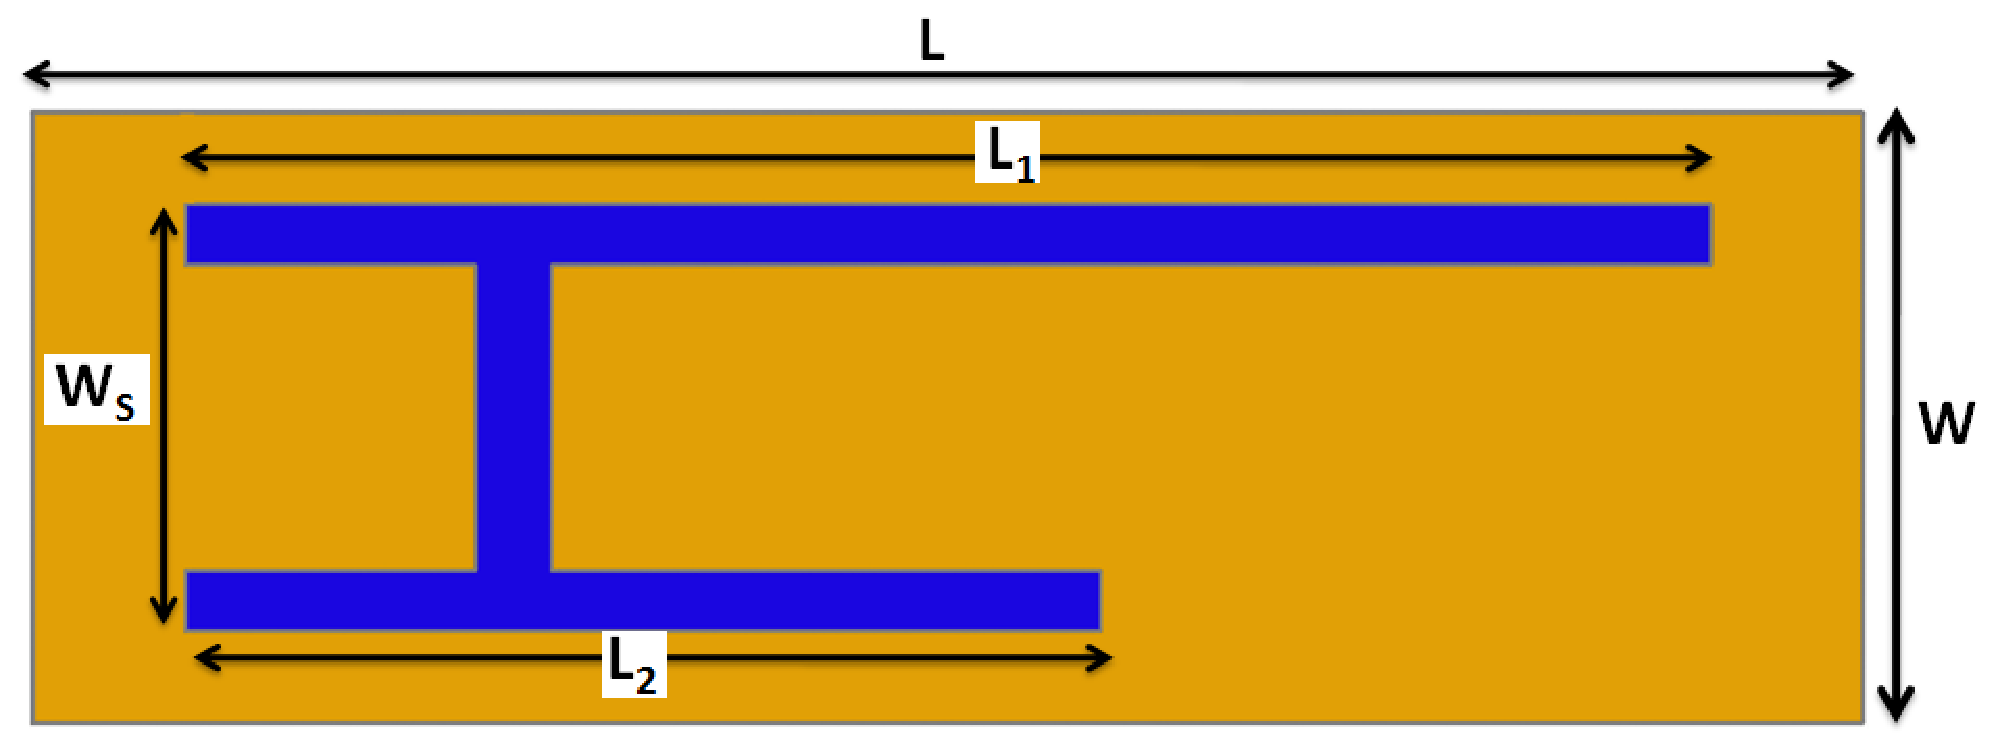
\includegraphics[width=0.7\linewidth]{bc-ant_top.eps}}\\
\subfigure[]{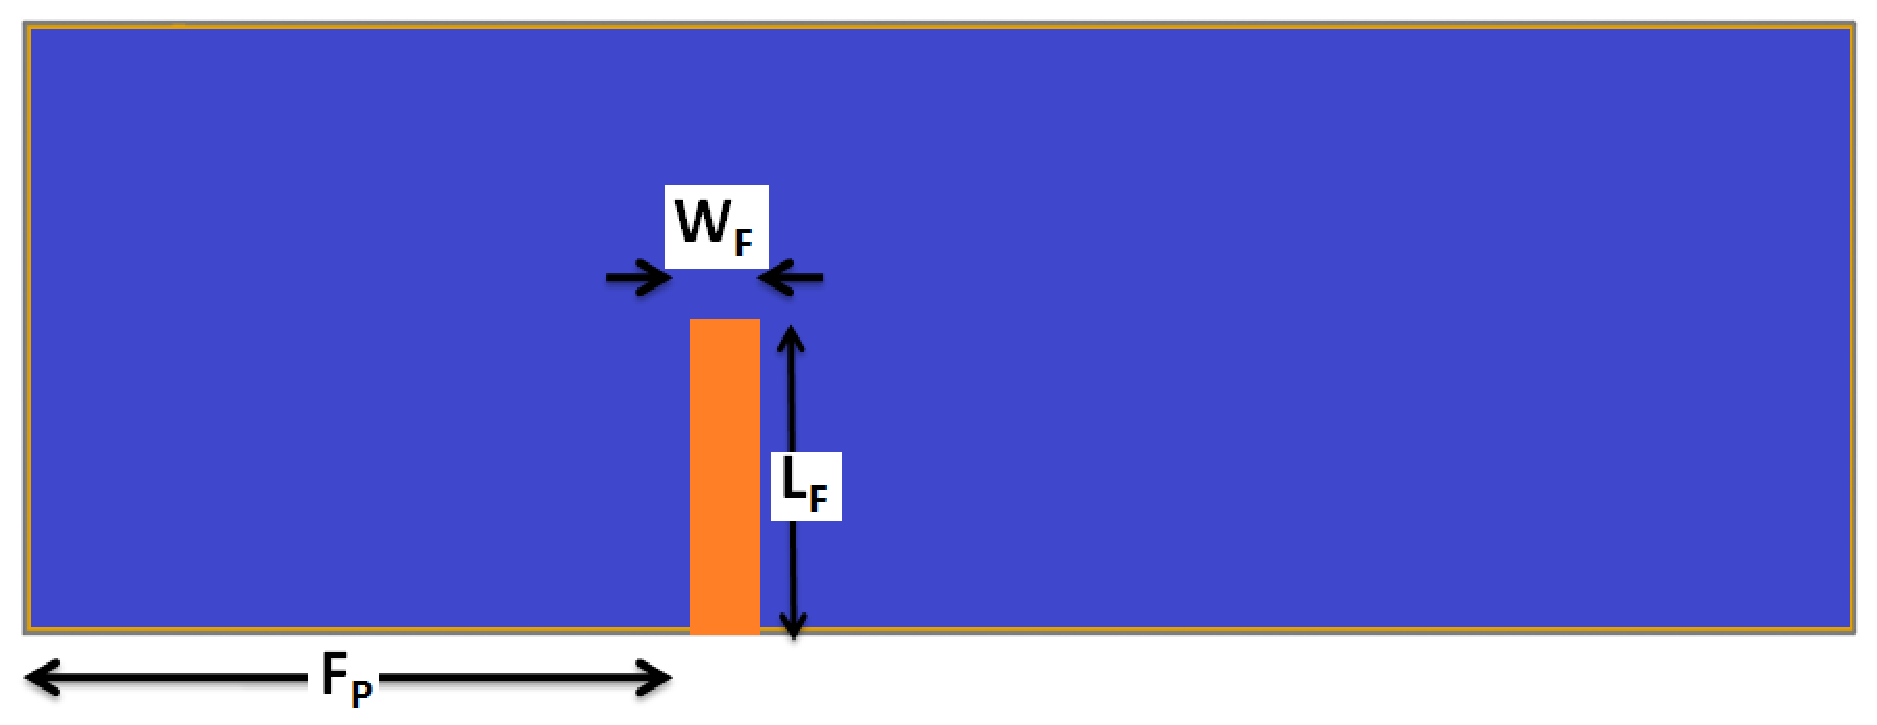
\includegraphics[width=0.7\linewidth]{bc-ant_back.eps}}\\
\caption{(a) Top view and (b) Bottom view of the example antenna}\label{h-shaped-topology}
\end{figure}

\begin{table}[h]
\centering
\caption{Dimensions of the test antenna} \label{tab-h-dim}
\label{tab:my-table}
\resizebox{0.5\textwidth}{!}{%
\begin{tabular}{|l|c|}
\hline
\textbf{Dimension} & \textbf{Value (mm)} \\ \hline
Length of the substrate ($L$) & 60 \\ \hline
Width of the substrate ($W$) & 20 \\ \hline
Length $L_1$ of the H-slot & 50 \\ \hline
Length $L_2$ of the H-slot & 30 \\ \hline
Width of the H-slot($W_S$) & 14 \\ \hline
\end{tabular}}
\end{table}

Optimizing the feed position of an antenna is an one-dimensional problem, that is, its DNA size is one. Since antenna simulation is a time-consuming task, the population size is kept small. In this case, the population size is five. The maximum number of generations is kept 50. The antenna is optimized to obtain its resonant frequencies at 2.4 GHz and 3.6 GHz. Hence, the cost function is derived as shown in Equation \ref{dual_cost}:

\begin{equation}\label{dual_cost}
\text{error}=\left|f_{r1}-2.4\times10^9\right|+\left|f_{r2}-3.6\times10^9\right|
\end{equation}

Here, $f_{r1}$ and $f_{r2}$ respectively are the first and the second resonant frequencies of the antenna. The resonant frequencies are obtained at the local minimum points of the S11 parameter plot. The python script saves the S11 parameter plot as a CSV file and then reads the file to find the minimum points of the S11 parameter.

The time required for running one simulation depends on a many of factors. If the antenna has a complex or circular geometry, the computation time is high. If the geometry of the antenna is simple, the computation time is relatively low. The computation time also depends on the frequency range over which the simulation is performed. The final antenna has a feed potion 35 mm.

The script interface of AEDT enables an user to create elements, change variables, run simulations and export the results to files. It is not possible to access the simulation results directly using the scripts. Further, the iron-python interface of AEDT lacks support for many python packages, such as SciPy, NumPy, Random, etc. that are crucial for implementing algorithms involving mathematical operations.

These problems are addressed by writing own programs for micro-tasks such as generating random numbers, dividing mathematical expressions into smaller arithmetic blocks, etc. In order to obtain the s11 parameters for evaluating the cost function,, the results are first exported to a CSV file and then read programmatically and parsed the data.

\section{Experimental Results} \label{c3sec_expt-res}
This section provides the details of the optimized antenna. The optimized H-shaped slot antenna is fabricated on a copper-FR4 PCB board. The fabricated antenna is shown in Fig. \ref{h-shaped-fab}. The performance of the antenna is evaluated from the return loss parameter (S11) plot and the far field radiation patter. In Fig. \ref{fig-s11-opt}, the simulated and the measured $S_{11}$ parameter plot of the antenna are shown. It is observed that the optimized dual-band antenna has resonant frequencies at 2.4 GHz and 3.6 GHz. The radiation patterns of the antenna at the two resonant frequencies are shown in Fig. \ref{fig-pattern}.

\begin{figure}
\centering
\subfigure[]{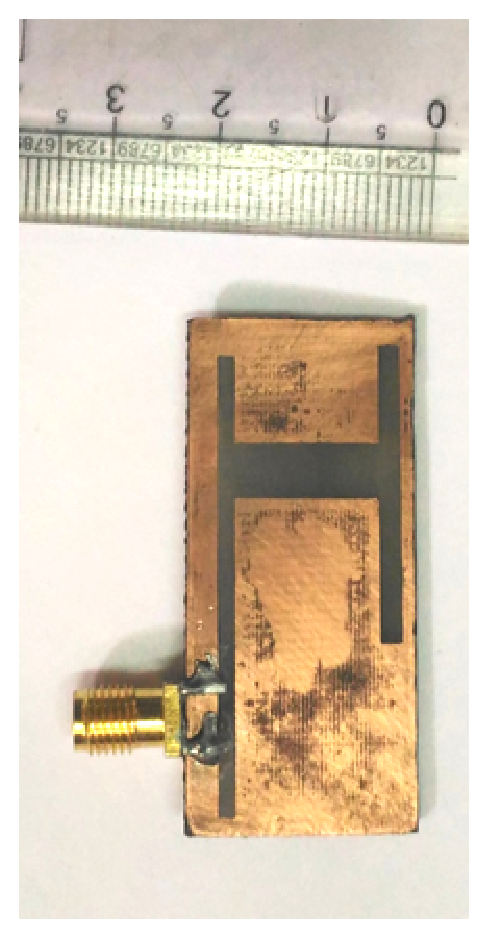
\includegraphics[width=0.3\linewidth]{bc-fab-front-h-slot.eps}}~~~
\subfigure[]{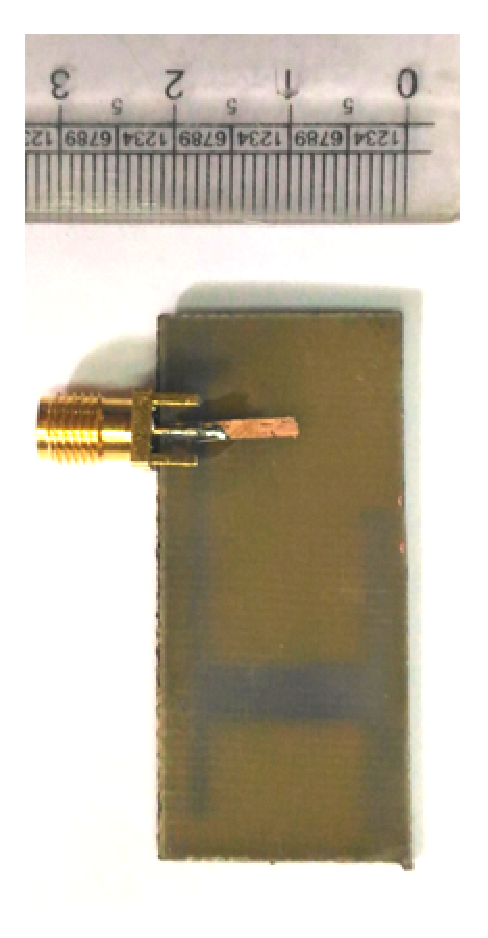
\includegraphics[width=0.3\linewidth]{bc-fab-back-h-slot.eps}}\\
\caption{(a) Top view and (b) Bottom view of the fabricated antenna}\label{h-shaped-fab}
\end{figure}

From Fig. \ref{fig-s11-opt}, it is observed that the antenna resonates at 2.4 GHz and 3.6 GHz. The simulated and the measured result shows a good agreement. This is possible because of the full-wave simulation used for computing the cost function. The full-wave simulation provides very high accuracy. This ensures minimum deviation between the optimized antenna for real-world application. The S11 parameter plot further shows that the antenna is useful for the ISM bands of 2.4 GHz and 3.6 GHz. The bandwidth of the antenna is about 200 MHz at the 2.4 GHz and about 700 MHz at the 3.6 GHz.

\begin{figure}
\centering
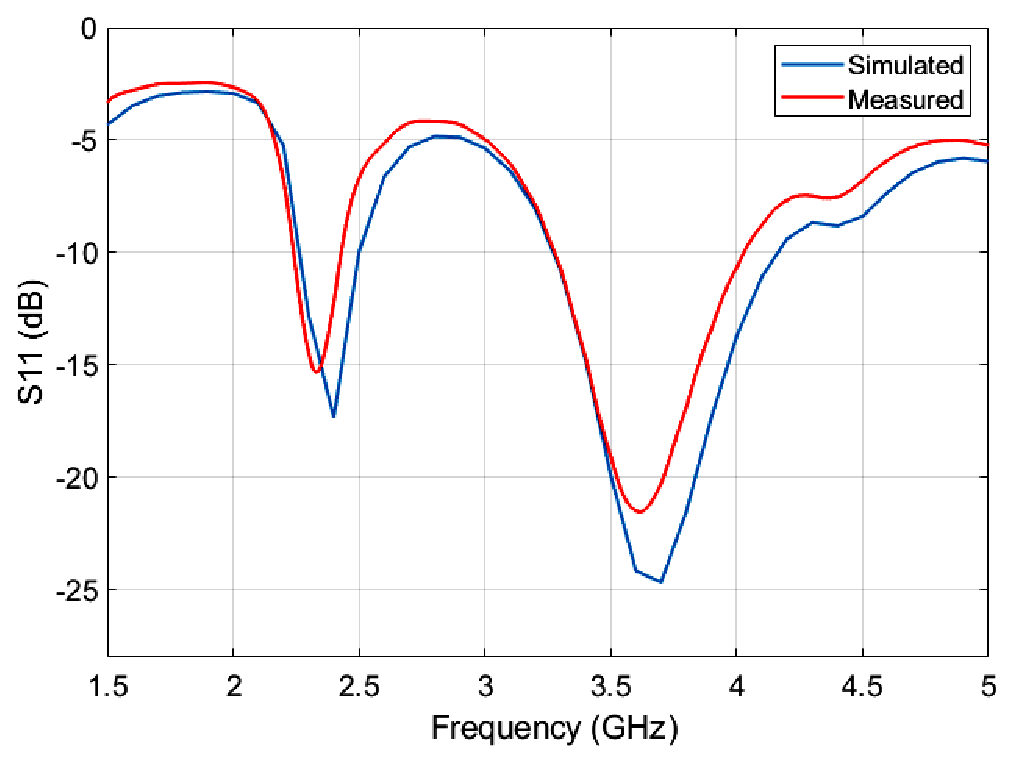
\includegraphics[width=0.7\linewidth]{bc-s11_res.eps}\\
\caption{Simulated and measured $S_{11}$ parameter plot of the optimized antenna}\label{fig-s11-opt}
\end{figure}

The radiation pattern of the antenna was not optimized. It is observed that the antenna has a far-field gain of 2 dBi in the direction of the major lobe ($\theta=0$) for both 2.4 GHz and 3.6 GHz. Thus, the antenna has almost the same sensitivity in this direction at both of its resonant frequency. However, the resonant frequency at 3.6 GHz is clearly is a higher order mode of the antenna and hence its radiation pattern has more than one major lobe.

\begin{figure}[h]
\centering
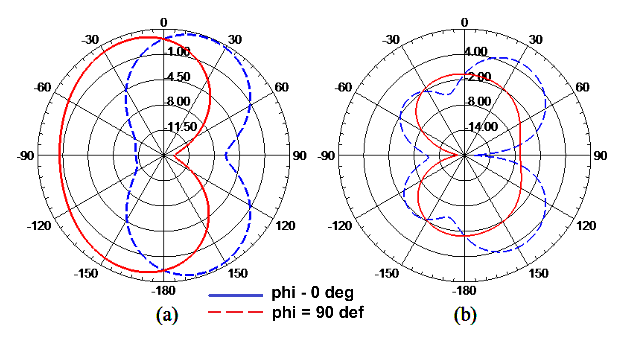
\includegraphics[width=0.7\linewidth]{bc-patterns.eps}\\
\caption{Far field radiation pattern of the proposed antenna at (a) 2.4 GHz and (b) 3.6 GHz}\label{fig-pattern}
\end{figure}

From the experimental results discussed, it is observed that the optimization algorithm is capable of meeting design criteria as specified in the cost function. However, the optimization algorithm cannot ensure that the other parameters of the antenna are also within conventionally acceptable limits. Constructing more complex cost functions may help in meeting multiple design goals. The high time requirement of full-wave techniques is the biggest drawback of this approach. To meet multiple design goals, it is important to tune multiple physical dimensions of the antenna. This leads to an exponential increase of the number of simulations to be performed.

\section{Conclusion}\label{c3sec_concl}
Genetic algorithm is one of the most popular bio-inspired optimization techniques. It has a wide range of application in various fields. There are many different implementations of this algorithm for various problems. An implementation of the genetic algorithm is presented for optimization of printed antenna with Ansys AEDT. The feed position of a H-shaped slot antenna is optimized with the proposed technique. The full-wave electromagnetic solver is used in each iteration of the optimization loop to calculate the cost function.

This approach guarantees a minimum difference between simulation and measurement results. However, the approach does not guarantee good performance of other electromagnetic parameters that may be desirable in a given case. Further, full-wave electromagnetic solvers require more time and computational resources as compared to other approximation based approaches. It is therefore not always feasible to optimize multiple dimensions of an antenna with this approach. The number of iterations required increases with the number of dimensions to be optimized. A time required for the optimization process in this case may range from several hours to several days depending upon the complexity of the design and the capacity of the computational hardware. However, the time required in this case is less compared to the optimetric tool that comes in-built with AEDT. The optimetric tool simulates the antenna for all possible values of the design parameters without any feedback loop. The feedback loop in genetic algorithm helps in significantly reducing the number of simulations required.

Here, the genetic algorithm is implemented using the Iron-Python script interface available with AEDT. This is a very minimal implementation of Python and lacks the support of various python packages that are vital for numerical computations of any kind. This  adds to the challenges in implementing soft-computing techniques such as genetic algorithm. There are other approaches where a more powerful computational tools such as Matlab is interfaced with the AEDT for better performance. The proposed approach requires less computational resources at the cost of an increased complexity of implementation. It can possibly speed up the optimization process in certain cases.
